\documentclass[conference]{IEEEtran}
\IEEEoverridecommandlockouts
\usepackage{cite}
\usepackage{amsmath,amssymb,amsfonts}
\usepackage{algorithmic}
\usepackage{graphicx}
\usepackage{textcomp}
\usepackage{xcolor}
\def\BibTeX{{\rm B\kern-.05em{\sc i\kern-.025em b}\kern-.08em
    T\kern-.1667em\lower.7ex\hbox{E}\kern-.125emX}}
    
    
\begin{document}

\title{Control of Solid State Transformer based on  Modular Multilevel Converters with Interconnecting Dual Active Bridges}
\author{\IEEEauthorblockN{Marcelo A. Perez\IEEEauthorrefmark{1},
Felipe Ruiz\IEEEauthorrefmark{1}, Jose R. Espinoza\IEEEauthorrefmark{2} and Mariusz Malinowski\IEEEauthorrefmark{3}}
\IEEEauthorblockA{\IEEEauthorrefmark{1}\textit{Department of Electronics}, \textit{Universidad Tecnica Federico Santa Maria}\\
Valparaiso, Chile \\
Email: marcelo.perez@usm.cl, felipe.ruizal@sansano.usm.cl}
\IEEEauthorblockA{\IEEEauthorrefmark{2}\textit{Department of Electrical Engineering}, \textit{Universidad de Concepcion}\\
Concepcion, Chile\\
Email: jose.espinoza@udec.cl}
\IEEEauthorblockA{\IEEEauthorrefmark{3}\textit{Institute of Control and Industrial Electronics}, \textit{Technical University of Warsaw}\\
Warsaw, Poland\\
Email: malin@isep.pw.edu.pl}%
}
 

\maketitle

\begin{abstract}
The increasing incorporation of energy storage and electric vehicles to the grid and the  injection of variable renewable energies and hybrid microgrids will impose an important challenge to the transformer design and operation. Solid state transformers  become a suitable alternative to address these issues due to the high controllability they perform. Particularly, modular solid state transformer are the preferred choice at distribution level due to the high voltage rating, reliability and fault tolerance they feature. In this paper a modular solid state transformer based on two modular multilevel converter connected by a series of isolated dual active bridges is proposed. The proposed topology is analyzed and mathematically modeled, and a suitable controller is designed. Simulations results shows the performance of the proposed topology and control scheme.
\end{abstract}



\section{Introduction}
 
Solid-state transformers (SST), provide several advantages over  conventional line frequency transformers such as low volume and weight, high  power density, high efficiency for light loads, transient and harmonics compensation, active voltage regulation \cite{7951721}, demand-side management, power factor control, voltage ride-through,  unbalance loads compensation  becoming an  intelligent element which can  improve the performance and power quality of power systems \cite{7497683}.

 

 
The basic theoretical concept of SST was proposed several decades ago  \cite{7575768}, but the development of multilevel converter topologies such as cascaded H bridge (CHB) and Modular Multilevel Converter (MMC) has allowed to increase the operating voltage levels, increase the reliability and provide fault tolerant operation due to the modular implementation \cite{5482117, Malinowski}. 


The MMC is one of the most versatile power converter topology which, due to its large voltage capability and high power quality of voltages and currents, has been employed mainly in HVDC transmission systems  \cite{6757004}. However,  it has been also  used  for  integration of HVDC   and  MVDC grids to the power system \cite{7482715, 7742996}, to improve the power distribution \cite{7460260}, to manage hybrid microgrids connection to the grid \cite{6584014}, as well as to connect and control renewable energy and storage systems to the power system \cite{7920367}.

Several modular SST structures have been proposed based on MMC. One of the common features of these structures is the use of  dual active bridges (DAB) to transfer power between submodules \cite{8430592}. Hence the reliability is increased because, if one of the submodules fails, the remaining submodules can still transfer power to the load  \cite{6661455}. 

In modular SST structures there are different types of interconection of submodules at the input and output sides. For distribution transformers the most common interconnection is input-series output-parallel (ISOP) in order to achieve high voltage at the input and large currents at the output \cite{7792816}. On the other hand, for interconnecting different distribution grids with similar operating voltages, the  input-series  output-series (ISOS) configuration can be used, exhibiting high voltage rating and reduced filter requirements at both sides \cite{7088624, 5739137}.

In ISOS configuration an unbalance of AC voltages in the series connection can occur, but it can be compensated directly in the modulation of each  converter \cite{6294454}. It is also possible to directly  control the input current and the balance of the capacitor voltages in the DAB by a coordinated modulation of the different stages \cite{5750052}.

The control these modular SST structures, it is possible to use similar current and voltage control structures developed for standard MMC because they are usually based on the equivalent voltage generated in each arm.  The AC currents are usually  controlled using a decoupled approach \cite{7047221}, the capacitor voltage is controlled  using also a decoupled strategy \cite{7094290}, while the power transfer in the DAB is controlled by the phase angle between AC voltages in the transformer terminals \cite{5762359}. The main consideration of the control system is focused on the voltage balance methods which must be coordinated with the power exchange control method of the DAB \cite{7927431}.

In this paper, an SST structure based on MMC in ISOS configuration interconnected by DABs is proposed. The converter is modeled and a control scheme is designed separating the control objectives by the different stages employing standard sorting techniques to keep the capacitor voltages of the MMC at a given level, decoupling control strategies for current control and a phase angle control for power transfer in the DAB.



\section{Solid State Transformer}
The proposed solid state transformer is composed of two MMCs connected through theirs submodules by means of a series of DABs as shown in Fig. \ref{fig:topology}. In this  topology the power is transmitted from the primary to the secondary in a distributed manner allowing to reduce the size of medium voltage transformer, increasing the efficiency and reducing the cost of magnetic elements.  Additional, it provides fault tolerant operation because each sub-module transmit only a small portion of the total power, if one of these modules fails it should be possible to work continuously, with only a small reduction in power,  preserving the full capabilities of modularity and availability of MMC. In this sense, compared to back-to-back MMC provides a modular transference of power increasing the availability of the SST and simplifying the design of the magnetic components due to the reduced current in each high frequency transformer.

Additionally, due to the ac and dc ports in each MMC, this topology can be connected either to AC or DC systems which is particularly useful for HVDC and  photovoltaic plants. Due to the similar voltages provided by the input and output MMCs this topology is intended to interconnect two systems instead of mimic a distribution transformer.


\begin{figure}[!t]
\centering
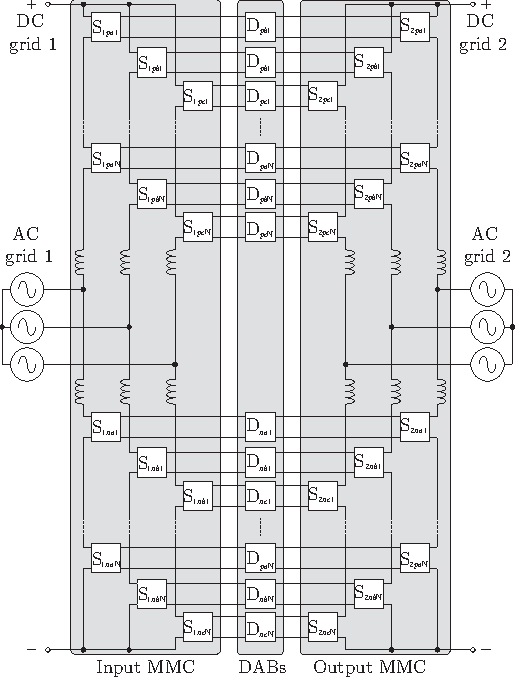
\includegraphics[width=\columnwidth]{images/topology.pdf}
\caption{Topology of the proposed Solid State Transformer.}
\label{fig:topology}
\end{figure}





\section{Mathematical Modeling}
A suitable mathematical model for the MMCs and the interconnecting DABs are given in this section in order to propose a control system in the next section.

\subsection{Modular Multilevel Converter}
The model of the MMC currents is obtained from \cite{7047221}, in which the arm currents are decomposed into three components (dc, ac and circulating) and a common mode voltage.

To obtain this model the voltages of the submodules are combined to generate the arm voltages, as shown in Fig. \ref{fig:MMC}, hence
\begin{align}
v_{xy}&=\sum_{i=1}^N v_{xyi}=\sum_{i=1}^N s_{xyi}v_{cxyi}
\end{align}
where $x=\{p,n\}$, $y=\{a,b,c\}$ and $i=\{1,...,N\}$.

Considering a matrix representation of arm voltages 
\begin{align}
\mathbf{V_{xy}}=
\left[\begin{array}{ccc}v_{pa}&v_{pb}&v_{pc}\\v_{na}&v_{nb}&v_{nc}\end{array}\right]
\end{align}
and arm currents
\begin{align}
\mathbf{I_{xy}}=
\left[\begin{array}{ccc}i_{pa}&i_{pb}&i_{pc}\\i_{na}&i_{nb}&i_{nc}\end{array}\right]
\end{align}
and applying the transformation proposed in \cite{7047221}, it  is possible to find a representation of the arm currents in terms of ac, dc and circulating current components as
\begin{align}
\mathbf{I_{xy}}=\mathbf{I_{o}}+\mathbf{I_{s}}+\mathbf{I_{z}}
\end{align}
each one having the following dynamic equations:
\begin{align}
(L+2L_{ac})\frac{d}{dt}\mathbf{I_{o}}+(r+2r_{ac})\mathbf{I_{o}}&=\mathbf{U_{o}}\\
(3L_{dc}+L)\frac{d}{dt}\mathbf{I_{s}}+(3r_{dc}+r)\mathbf{I_{s}}&=\mathbf{U_{s}}\\
L\frac{d}{dt}\mathbf{I_{z}}+r\mathbf{I_{z}}&=\mathbf{U_{z}}
\end{align}

\begin{figure}[!t]
\centering
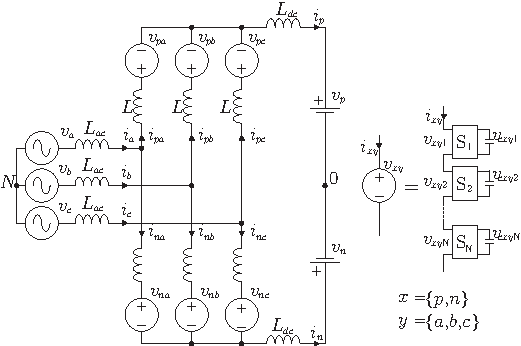
\includegraphics[]{images/MMC.pdf}
\caption{Modular Multilevel Converter.}
\label{fig:MMC}
\end{figure}

The details in the current modelling are found in \cite{7047221} and there are not explained here due to space constrains. The common mode current is zero because there is no connection between the DC neutral and AC neutral points in Fig. \ref{fig:topology}. 
The common mode voltage between these two points is given by
\begin{align}
\mathbf{V_{N0}}&=\mathbf{U_{m}}
\end{align}
The input of the coupled model $\mathbf{U_{xy}}$ is given by the combination of dc ($\mathbf{V_{x}}$), ac ($\mathbf{V_{y}}$) and arm ($\mathbf{V_{xy}}$) voltages,
\begin{align}
\mathbf{U_{xy}}&=\mathbf{V_{x}}-\mathbf{V_{y}}-\mathbf{V_{xy}}
\end{align}
The same transformation used for the currents is applied to this input obtaining 
\begin{align}
\mathbf{U_{o}}&=\mathbf{P_2}\mathbf{U_{xy}}\mathbf{Q_3}=-\mathbf{V_{y}}-\mathbf{P_2}\mathbf{V_{xy}}\mathbf{Q_3}\\
\mathbf{U_{s}}&=\mathbf{Q_2}\mathbf{U_{xy}}\mathbf{P_3}=\mathbf{V_{x}}-\mathbf{Q_2}\mathbf{V_{xy}}\mathbf{P_3}\\
\mathbf{U_{z}}&=\mathbf{Q_2}\mathbf{U_{xy}}\mathbf{Q_3}=-\mathbf{Q_2}\mathbf{V_{xy}}\mathbf{Q_3}\\
\mathbf{U_{m}}&=\mathbf{P_2}\mathbf{U_{xy}}\mathbf{P_3}=-\mathbf{P_2}\mathbf{V_{xy}}\mathbf{P_3}
\end{align}
It is possible to notice that each arm current component and common mode voltage is controlled by the respective component of the arm voltage generated by the submodules.


On the other hand, the model of the MMC currents are obtained from \cite{7094290}, in which the dynamical response of the capacitor voltage in each submodule is
\begin{align}
C\frac{dv_{cxyi}}{dt}+\frac{v_{cxyi}}{R}=i_{xy}s_{xyi}
\end{align}
multiplying this equation by the capacitor voltage it is possible to obtain the arm energy model
\begin{align}
\frac{d e_{cxy}}{dt}+\frac{2}{RC}e_{cxy}=i_{xy}v_{xy}
\end{align}
where $e_{cxyi}=\frac{1}{2}Cv_{cxyi}^2$. The energy of each arm can be written in matrix notation  as
\begin{align}
\frac{d}{dt}\mathbf{E_{c}}+\frac{2}{RC}\mathbf{E_{c}}=\mathbf{I_{xy}}\odot \mathbf{V_{xy}}
\end{align}
where $\odot$ is the element by element multiplication and
\begin{align}
\mathbf{E_{c}}=
\left[\begin{array}{ccc}e_{cpa}&e_{cpb}&e_{cpc}\\e_{cna}&e_{cnb}&e_{cnc}\end{array}\right]
\end{align}

Considering the ac voltage  as a disturbance and the dc voltage  as constant, the dynamic equations of the energy are
\begin{align}
\frac{d}{dt}\mathbf{E_s}\!+\!\frac{2}{RC}\mathbf{E_s}&=\!-\mathbf{U_m}\odot\mathbf{I_s}\label{eq:Es}\\
\frac{d}{dt}\mathbf{E_o}\!+\!\frac{2}{RC}\mathbf{E_o}&=\!\mathbf{V_x}\odot\mathbf{I_z}\\ 
\frac{d}{dt}\mathbf{E_z}\!+\!\frac{2}{RC}\mathbf{E_z}&=\!\mathbf{V_x}\odot\mathbf{I_o}\\
\frac{d}{dt}\mathbf{E_m}\!+\!\frac{2}{RC}\mathbf{E_m}&=\!\mathbf{V_x}\odot\mathbf{I_s}\label{eq:Em}
\end{align}

Therefore, according to \cite{7094290} it is possible to control the different components of the energy, which in turn control the balance of capacitor voltages, using the references of circulating, ac and dc currents, as well as the common mode voltage. 


\subsection{Power Transfer Module}
Each submodule $xyi$ is modeled with a converter connected to the input MMC, a power transfer DAB and a converter connected to the output MMC as shown in Fig. \ref{fig:DAB}.


\begin{figure}[!t]
\centering
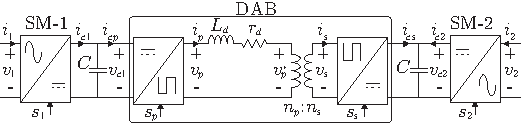
\includegraphics[]{images/DAB.pdf}
\caption{Power Transfer Submodule.}
\label{fig:DAB}
\end{figure}

At the input MMC, the dynamic of the submodule capacitor voltage $v_{c1}$ is given by
\begin{align}\label{eq:inputMMC}
C\frac{d}{dt}v_{c1}+\frac{v_{c1}}{R}&=i_{c1}-i_{cp}
\end{align}
where $C$ and $R$ are the capacitance and parallel parasitic resistance, respectively, the output current of the converter is 
\begin{align}
i_{c1}&=s_{1}i_{1}
\end{align}
an the input current of the DAB is
\begin{align}
i_{cp}=s_{p}i_{p}
\end{align}

The  dynamic of the output MMC capacitor voltage $v_{c2}$ is given by
\begin{align}\label{eq:outputMMC}
C\frac{d}{dt}v_{c2}+\frac{v_{c2}}{R}&=i_{cs}+i_{c2}
\end{align}
where the output current of the DAB is
\begin{align}
i_{cs}=s_{s} i_{s}
\end{align}
and the input current of the converter is
\begin{align}
i_{c2}&=s_{2}i_{2}
\end{align}

The dynamic model of the primary current in the DAB is
\begin{align}\label{eq:DAB}
L_{d}\frac{d}{dt}i_{p}+R_d i_{p}=v_{p}-v_{p}^{'}
\end{align}
where $L_p$ and $r_p$ are the inductance and resistance of the transformer, the voltage at the primary is 
\begin{align}
v_{p}=s_{p}v_{c1}
\end{align}
and voltage at the secondary is
\begin{align}
v_{s}=s_{s}v_{c2}
\end{align}
Considering an ideal transformer, where the relation between voltages and currents are $\frac{v_{p}^{'}}{n_p}=\frac{v_{s}}{n_s}$ and $n_pi_p=n_si_s$ and solving  equation (\ref{eq:DAB}) is possible to find the fundamental frequency component of the DAB current as
\begin{align}
L_{p}\frac{d}{dt}i_{p}\!+\!r_p i_{p}\!=\!\frac{4}{\pi}V_{c1}\sin(\omega_p t)\!-\!\frac{n_p}{n_s}\frac{4}{\pi}V_{c2}\sin(\omega_p t\!-\!\phi)
\end{align}
where $\phi$ is the angle between the switching signal of the input and output converters in the DAB. Considering the fundamental component of the current
\begin{align}
i_p&=I_{p}\sin(\omega_p t-\alpha)=I_{pd}\sin(\omega_p t)-I_{pq}\cos(\omega_p t)
\end{align}
the direct and quadrature components are
\begin{align}
I_{pd}&=\frac{4V_{c1}}{\pi Z_p}\left(\cos(\gamma)-\frac{n_p}{n_s}\frac{V_{c1}}{V_{c2}}\cos(\gamma+\phi)\right)\\
I_{pq}&=\frac{4V_{c1}}{\pi Z_p}\left(\sin(\gamma)-\frac{n_p}{n_s}\frac{V_{c1}}{V_{c2}}\sin(\gamma+\phi)\right)
\end{align}

where $Z_p=\sqrt{r_p^2+\omega_p^2L_p^2}$ and $\gamma=\arctan(\omega_pL_p/r_p)$. 

Using this model is possible to design a power transfer controller as shown in the next section.



\section{Proposed Control system}
The proposed control system is composed of three control loops, one for the input MMC, one for the DAB and one for the output MMC, as shown in Fig. \ref{fig:control}.



\begin{figure}[!t]
\centering
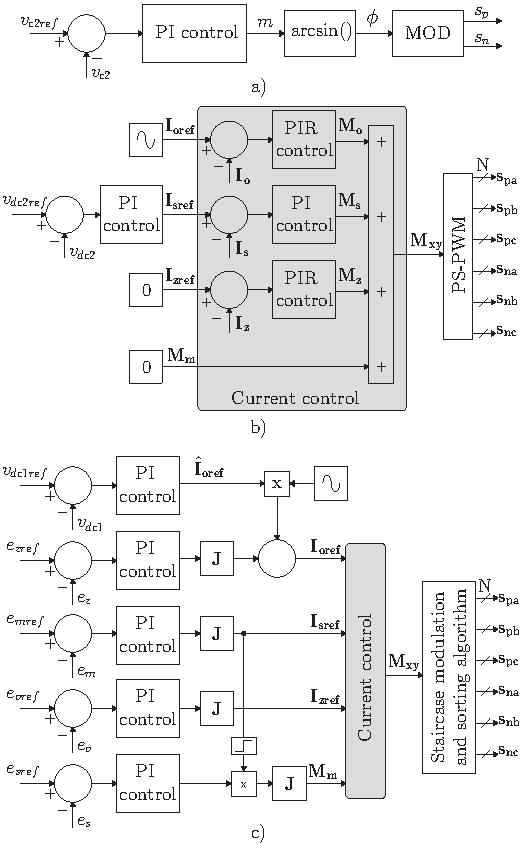
\includegraphics[width=\columnwidth]{images/Control2.pdf}
\caption{Proposed control scheme. a) DAB Control scheme. b) Output MMC control scheme. c) Input MMC control scheme.}
\label{fig:control}
\end{figure}


\subsection{DAB Control Scheme}
Considering $i_{c2}$ as a disturbance equation (\ref{eq:outputMMC}) can be expressed
\begin{align}
C\frac{dv_{c2}}{dt}+\frac{v_{c2}}{R}&=s_s\frac{n_p}{n_s}i_p
\end{align}
Multiplying by the voltage capacitor 
\begin{align}
\frac{C}{2}\frac{dv_{c2}^2}{dt}+\frac{v_{c2}^2}{R}&=v_s\frac{n_p}{n_s}i_p=p_s
\end{align}
which can be write in terms of the energy by
\begin{align}
\frac{de_{c2}}{dt}+\frac{2}{RC}e_{c2}&=p_s
\end{align}
Replacing the secondary voltage and primary current by the fundamental expressions given by
\begin{align}
i_p&=I_p\sin(\omega_p t-\alpha)
\end{align}
\begin{align}
v_s=\frac{4}{\pi}V_{c2}\sin(\omega_p t-\phi)
\end{align}
The expression of the power in the capacitor becomes
%\begin{align}
%p_s&=\frac{n_p}{n_s}\frac{4}{\pi}V_{c2}I_p\sin(\omega_p t-\phi)\sin(\omega_p t-\alpha)
%\end{align}
\begin{align}
p_s&=\frac{n_p}{n_s}\frac{2}{\pi}V_{c2}I_p(\cos(\alpha-\phi))-\cos(2\omega_p t-\phi-\alpha))
\end{align}
The first term of the right side represents the average charging value while the second  is sinusoidal term which charges and discharges the capacitor every cycle. Therefore, the dynamics of the capacitor voltage can be expressed as
%\begin{align}
%p_s&=\frac{n_p}{n_s}\frac{2}{\pi}V_{c2}I_p\cos(\alpha-\phi)
%\end{align}
\begin{align}
p_s&=\frac{n_p}{n_s}\frac{2}{\pi}V_{c2}(I_{pd}\cos(\phi)+I_{pq}\sin(\phi))
\end{align}
replacing the components of the current results
%\begin{align}
%p_s&=\frac{n_p}{n_s}\frac{8}{\pi^2}\frac{V_{c2}}{Z_p^2}\left( 
% V_{c1}(r_p\cos(\phi)\!+\!\omega_pL_p\sin(\phi))\! -\!\frac{n_p}{n_s}V_{c2}r_p
% \right)
%\end{align}
%or
\begin{align}
p_s&=\frac{n_p}{n_s}\frac{8}{\pi^2}\frac{V_{c2}}{Z_p}\left( 
 V_{c1}\cos(\phi-\gamma)-\frac{n_p}{n_s}V_{c2}\cos(\gamma)
 \right)
\end{align}
Considering $r_p<<\omega_pL_p$, hence $Z_p\approx\omega_pL_p$, $\gamma\approx\pi/2$, and 
\begin{align}
p_s&\approx\frac{n_p}{n_s}\frac{8}{\pi^2}\frac{V_{c2} V_{c1}}{\omega_pL_p}
\sin(\phi)
\end{align}

As can be seen from the previous equation the  power required to charge and discharge the capacitor in the output MMC is proportional to the angle between square waves at the input and output converters of the DAB.

Therefore, to control the capacitor voltage of the output MMC a lineal controller followed by an $\arcsin()$ function is used, as shown in Fig. \ref{fig:control} a).




\subsection{Output MMC controller}
In the output MMC the capacitor voltages are considered constant because they are controlled by the DAB controller. Therefore in this MMC it is required to control only the currents.
 
From the MMC model shown in the previous section, considering a constant capacitor value, it is possible to obtain the following transfer functions
\begin{align}
\mathbf{I_z}&=\frac{-NV_c}{L s+r}\,\mathbf{M_z}\\
\mathbf{I_s}&=\frac{-NV_c}{(3L_{dc}+L)s+(3r_{dc}+r)}\,\mathbf{M_s}\\
\mathbf{I_o}&=\frac{-NV_c}{(L+2L_{ac})s+(r+2r_{ac})}\,\mathbf{M_o}
\end{align}
where $\mathbf{M_z}$, $\mathbf{M_s}$ and $\mathbf{M_o}$ are the modulation indexes for the circulating, dc and ac current components, respectively. Considering these first order linear transfer functions, a set of three linear PI controller are used. The references for the ac component are generated arbitrarily but they can be generated from an external  power quality controller, for example. The dc current reference is generated from a PI control which is set to kept the DC voltage of the output MMC at a given reference level.  The circulating current reference, as well as the common mode modulation index, are set to zero. The complete control method is shown in Fig. \ref{fig:control} b).


\subsection{Input MMC controller}
The input MMC controller is composed of two stages. The first stage controls the circulating, ac and dc current and also the common mode voltage using the same structure shown for the output MMC. The main difference from the output MMC is the capacitor voltage is not fixed in this case and must be controlled by defining proper references for these currents and voltage.

In order to obtain these references an energy controller is employed based on the model of the capacitor energies of the MMC, shown in the previous section.  

According to the equations (\ref{eq:Es})-(\ref{eq:Em}) of the model,  $\mathbf{I_s}$ is used to control  $\mathbf{E_m}$, hence it becomes a parameter to control  $\mathbf{E_s}$, which must be controlled by  $\mathbf{U_m}$. The control of  $\mathbf{E_o}$ and $\mathbf{E_z}$ is perform using the variables  $\mathbf{I_z}$ and $\mathbf{I_o}$, respectively. 

Considering that $\mathbf{I_s}$ is a matrix with values $I_{dc}/3$ and $\mathbf{V_x}$is a matrix with values $V_{dc}/2$ and both matrix have the same structure, the models for energy control becomes
\begin{align}
\mathbf{E_s}&=F(s)\,\mathbf{J}\mathbf{U_m}\\
\mathbf{E_o}&=F(s)\,\mathbf{J}\mathbf{I_z}\\ 
\mathbf{E_z}&=F(s)\,\mathbf{J}\mathbf{I_o} \\
\mathbf{E_m}&=F(s)\,\mathbf{J}\mathbf{I_s}
\end{align}
where  
\begin{align}
\mathbf{J}=\left[\begin{array}{cc}1&0\\0&-1\end{array}\right]
, \text{and}\:\:\: F(s)=\frac{V_{dc}/2}{s+\frac{2}{RC}}
\end{align}

The complete control system is shown in Fig. \ref{fig:control} c). In this figure it is possible to notice the sign of the dc current reference is used to multiply the reference of $\mathbf{M_m}$ to compensate the dynamics if this current change its sign as shown in eq. (\ref{eq:Es}).

This example shows two ac systems interconnected, if one ac system is connected to a dc system the PI controller of $v_{dc1}$ in Fig. \ref{fig:control} c) must be connected to the $\mathbf{I_{sref}}$ instead of  $\mathbf{I_{sref}}$.

\begin{figure}[!t]
\centering
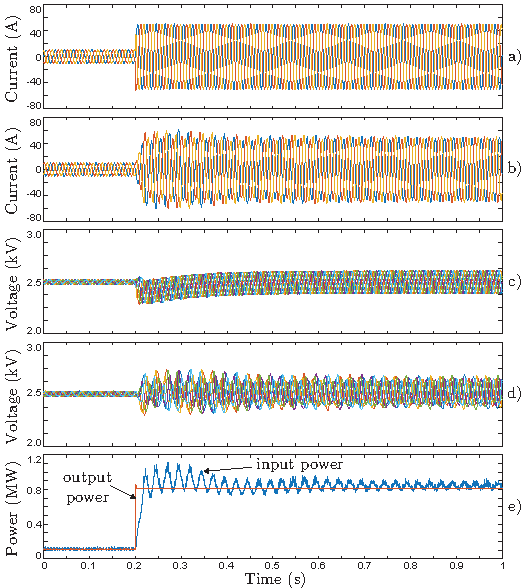
\includegraphics[width=\columnwidth]{images/results01-comprimido.pdf}
\caption{Simulation results of a step change in the output current reference. a) Output current. b) Input current. c) Output capacitor voltage. d) Input capacitor voltage. e) Input and output power.}
\label{fig:results01}
\end{figure}


\section{Results}
The proposed topology of SST is simulated and the control scheme implemented. Due to the linear and first order models found for all the converter dynamics, PI controllers designed by pole placement are used.

Fig. \ref{fig:results01} shows the results of a step change in the output current reference. Fig.  \ref{fig:results01} a) shows the three-phase output current which changes from 10A to 50A with a very fast dynamic response. The input current shown in Fig.  \ref{fig:results01} b) changes from 11A to 52A following the requirements of the load, however this change is slower and presents a small overshoot.  The capacitor voltages of the input and output MMC are controlled at the reference level  as shown in Fig.  \ref{fig:results01} c) and d), respectively.  The capacitor voltage of the output MMC shows a close balance among them but a larger deviation from the reference, due to the DAB control of the output MMC capacitor voltages. On the other hand,  the capacitor voltage of the input MMC  are not perfectly balance but the deviation from the reference is smaller due to the voltage balance control scheme of the input MMC. In Fig. \ref{fig:results01} e) are shown the input and output power. It can be seen that the output power changes very fast following the dynamical response of the current but the input power changes slower, presenting an oscillation and a steady state value larger than the output which difference correspond to the losses of the converter.   




Fig. \ref{fig:results02} shows a zoom of voltages and current at the moment of the step changes. It is possible to notice the output current changes and stabilizes very fast at the reference value keeping during all the process the unitary power factor as shown in Fig. \ref{fig:results02} a). The input current changes with an oscillation which is due to the dynamic response associated to the capacitor voltage control.  The current angle is controlled generating a unitary power factor as shown in Fig. \ref{fig:results02} b).

\begin{figure}[!t]
\centering
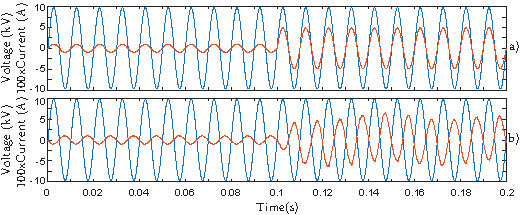
\includegraphics[width=\columnwidth]{images/results02.pdf}
\caption{Zoom of a step change in the output current reference. a) Output AC voltage (blue) and current (red). b) Input AC voltage (blue) and current (red).}
\label{fig:results02}
\end{figure}



 \section{Conclusions}
The series-input series-output SST based on MMC provides a high power quality interconnection between two systems and a high reliability due to the modular power transfer. The proposed control scheme separates the control objectives in three: output MMC current, output MMC capacitor voltage and input MMC current, each one controlled by the output MMC, interconnecting DAB and input MMC, respectively. From the results it is possible to notice the dynamical response of the output current is very fast, mainly due to the constant capacitor voltage imposed by the DAB. At the input the current dynamic is slower and oscillating due to the unbalances  in the capacitor voltage. In both cases, the current angle reference is  followed. 



\section*{Acknowledgment}
This work was supported by Fondecyt 1181839, by MEC 80150050, by SERC Chile (CONICYT/FONDAP/15110019) and by AC3E (CONICYT/FB0008). 




\bibliographystyle{IEEEtran}
\bibliography{references}
\vspace{12pt}
\end{document}
